\section{Problem Analysis}\label{sec:problem-analsysis}

	As mentioned in Section \ref{sec:purpose} this project aims on developing a functional brake test bench. Based on the \textit{SAE J2522} \cite{sae} and considering some instrumentation engineering concepts the project solution can be divided in the structure showed in Figure \ref{fig:projectProblem}.
	
	\begin{figure}[htbp]
		\centering
			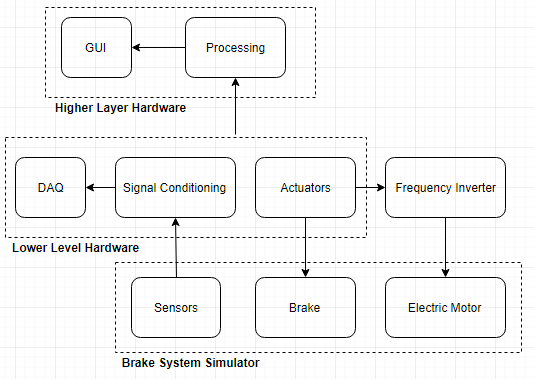
\includegraphics[scale=0.9]{figuras/fig-projectProblem}
		\caption{Project Problem Depuration \cite{projectProblem}}
		\label{fig:projectProblem}
	\end{figure}
	
	The explanation of the structure of Figure \ref{fig:projectProblem} will be explained in Sections \ref{ssec:brakeSystemSimulator} to \ref{ssec:solutionOverview}.

	\subsection{Brake System Simulator}\label{ssec:brakeSystemSimulator}
		
		The \textit{Brake System Simulator} block as the name says comprehends the hardware responsible for simulating the environment of a brake system, the two basic components are the \textit{Brake} component itself (in this case being a disc brake system) and a \textit{Electric Motor} to accelerate the rotor in order to simulate the speed a vehicle wheel might be submitted. A \textit{Sensors} block was also added, without acquiring a physical/mechanical quantities such as temperature and pressure, a brake test would be useless because no possible technical analysis could be done afterwards. The \textit{Sensors} block was placed inside the \textit{Brake System Simulator} block because the sensors and transducers will be placed arround the components of this major block.

	\subsection{Lower Layer Hardware}\label{ssec:lowerLayerlHardware}

		This layer of hardware will make the translation from physical/mechanical quantities to computer data, \textit{i.e.}, converting physical/mechanical quantities to voltage and than to bytes of information and also on the opposite way (bytes to voltage and voltage to physical/mechanical quantities). \textit{Sensors} signals are not always ready to read, as mentioned in Section \ref{sec:instrumentationEngineering}, Instrumentation Engineering also involves doing \textit{Signal Conditioning} to adapt sensor signals. The \textit{DAQ} block was inserted in order to demonstrate that there is the need for a solution to capture the sensors signals. \textit{Actuators} block are responsible to adapt the commands from upper layers to control the hardware. The \textit{Frequency Inverter} is already a more specific detail of the solution, but it was included here because most electric motors work with triphasic power and this device is fundamental to control them.

	\subsection{Higher Layer Hardware}\label{ssec:higherLayerlHardware}
	
		This layer of hardware although represented in a quite simple way in Figure \ref{fig:projectProblem} will probably involve the most dense code. This is because this layer needs to do all the heavy data processing, \textit{i.e.}, converting and dealing with the information that flows through all the structure. The \textit{GUI} block is the one responsible for acquiring and displaying computer information in a human-friendly format.

	\subsection{Solution Overview}\label{ssec:solutionOverview}

	Table \ref{tab:informationTranslation} shows the basic functon of each block on Figure \ref{fig:projectProblem}.

	\begin{table}[h!]
		\centering
		\caption{Blocks functionality}
		\label{tab:informationTranslation}
		\begin{tabular}{|l|l|}
			\hline
			\textbf{Block} & \textbf{Function} \\ \hline
			\textit{Sensors} & Convert physical quantities to electrical signals \\ \hline
			\textit{Signal Conditioning} & Adapt sensors electrical signals to best suit DAQ \\ \hline
			\textit{DAQ} & Converts electrical signals to computes bytes \\ \hline
			\textit{Actuators} & Convert voltage levels to physical/mechanical quantities \\ \hline
			\textit{Frequency Inverter} & Controls a triphasic motor speed \\ \hline
			\textit{Processing} & Control and process data flow \\ \hline
			\textit{GUI} & Displays/acquire information in a human-friendly format \\ \hline
		\end{tabular}
	\end{table}
